%
\section{The Fundamentals Behind StdRegions}
\label{sec:stdregions-fundamentals}

The idea behind standard regions can be traced back to one of the fundamental principles we learn in calculus: differentiation and integrating
on arbitrary regions are often difficult; however, differentiation and integration have been worked out on canonical (straight-sided or planar-sided), 
right-angled, coordinate aligned domains.   In the case of {\nek}, we do not need to work on truly arbitrary domains, but rather on seven
fundamental domains:  segments in 1D, triangles and quadrilaterals in 2D, and tetrahedra, hexahedra, prisms and pyramids in 3D.  Since
{\nek} deals with polynomial methods, the natural domain over which reference elements should be build is $[-1,1]$ as this is the
interval over which Jacobi Polynomials are defined and over which Gaussian quadrature is defined \cite{CanutoHQZ87}.  We show in
Figure \ref{stdregions:refelement} a pictorial representation of the standard segment, standard quadrilateral (often shorthanded quad) and
standard triangle.  


\begin{figure}[htb]
\centering
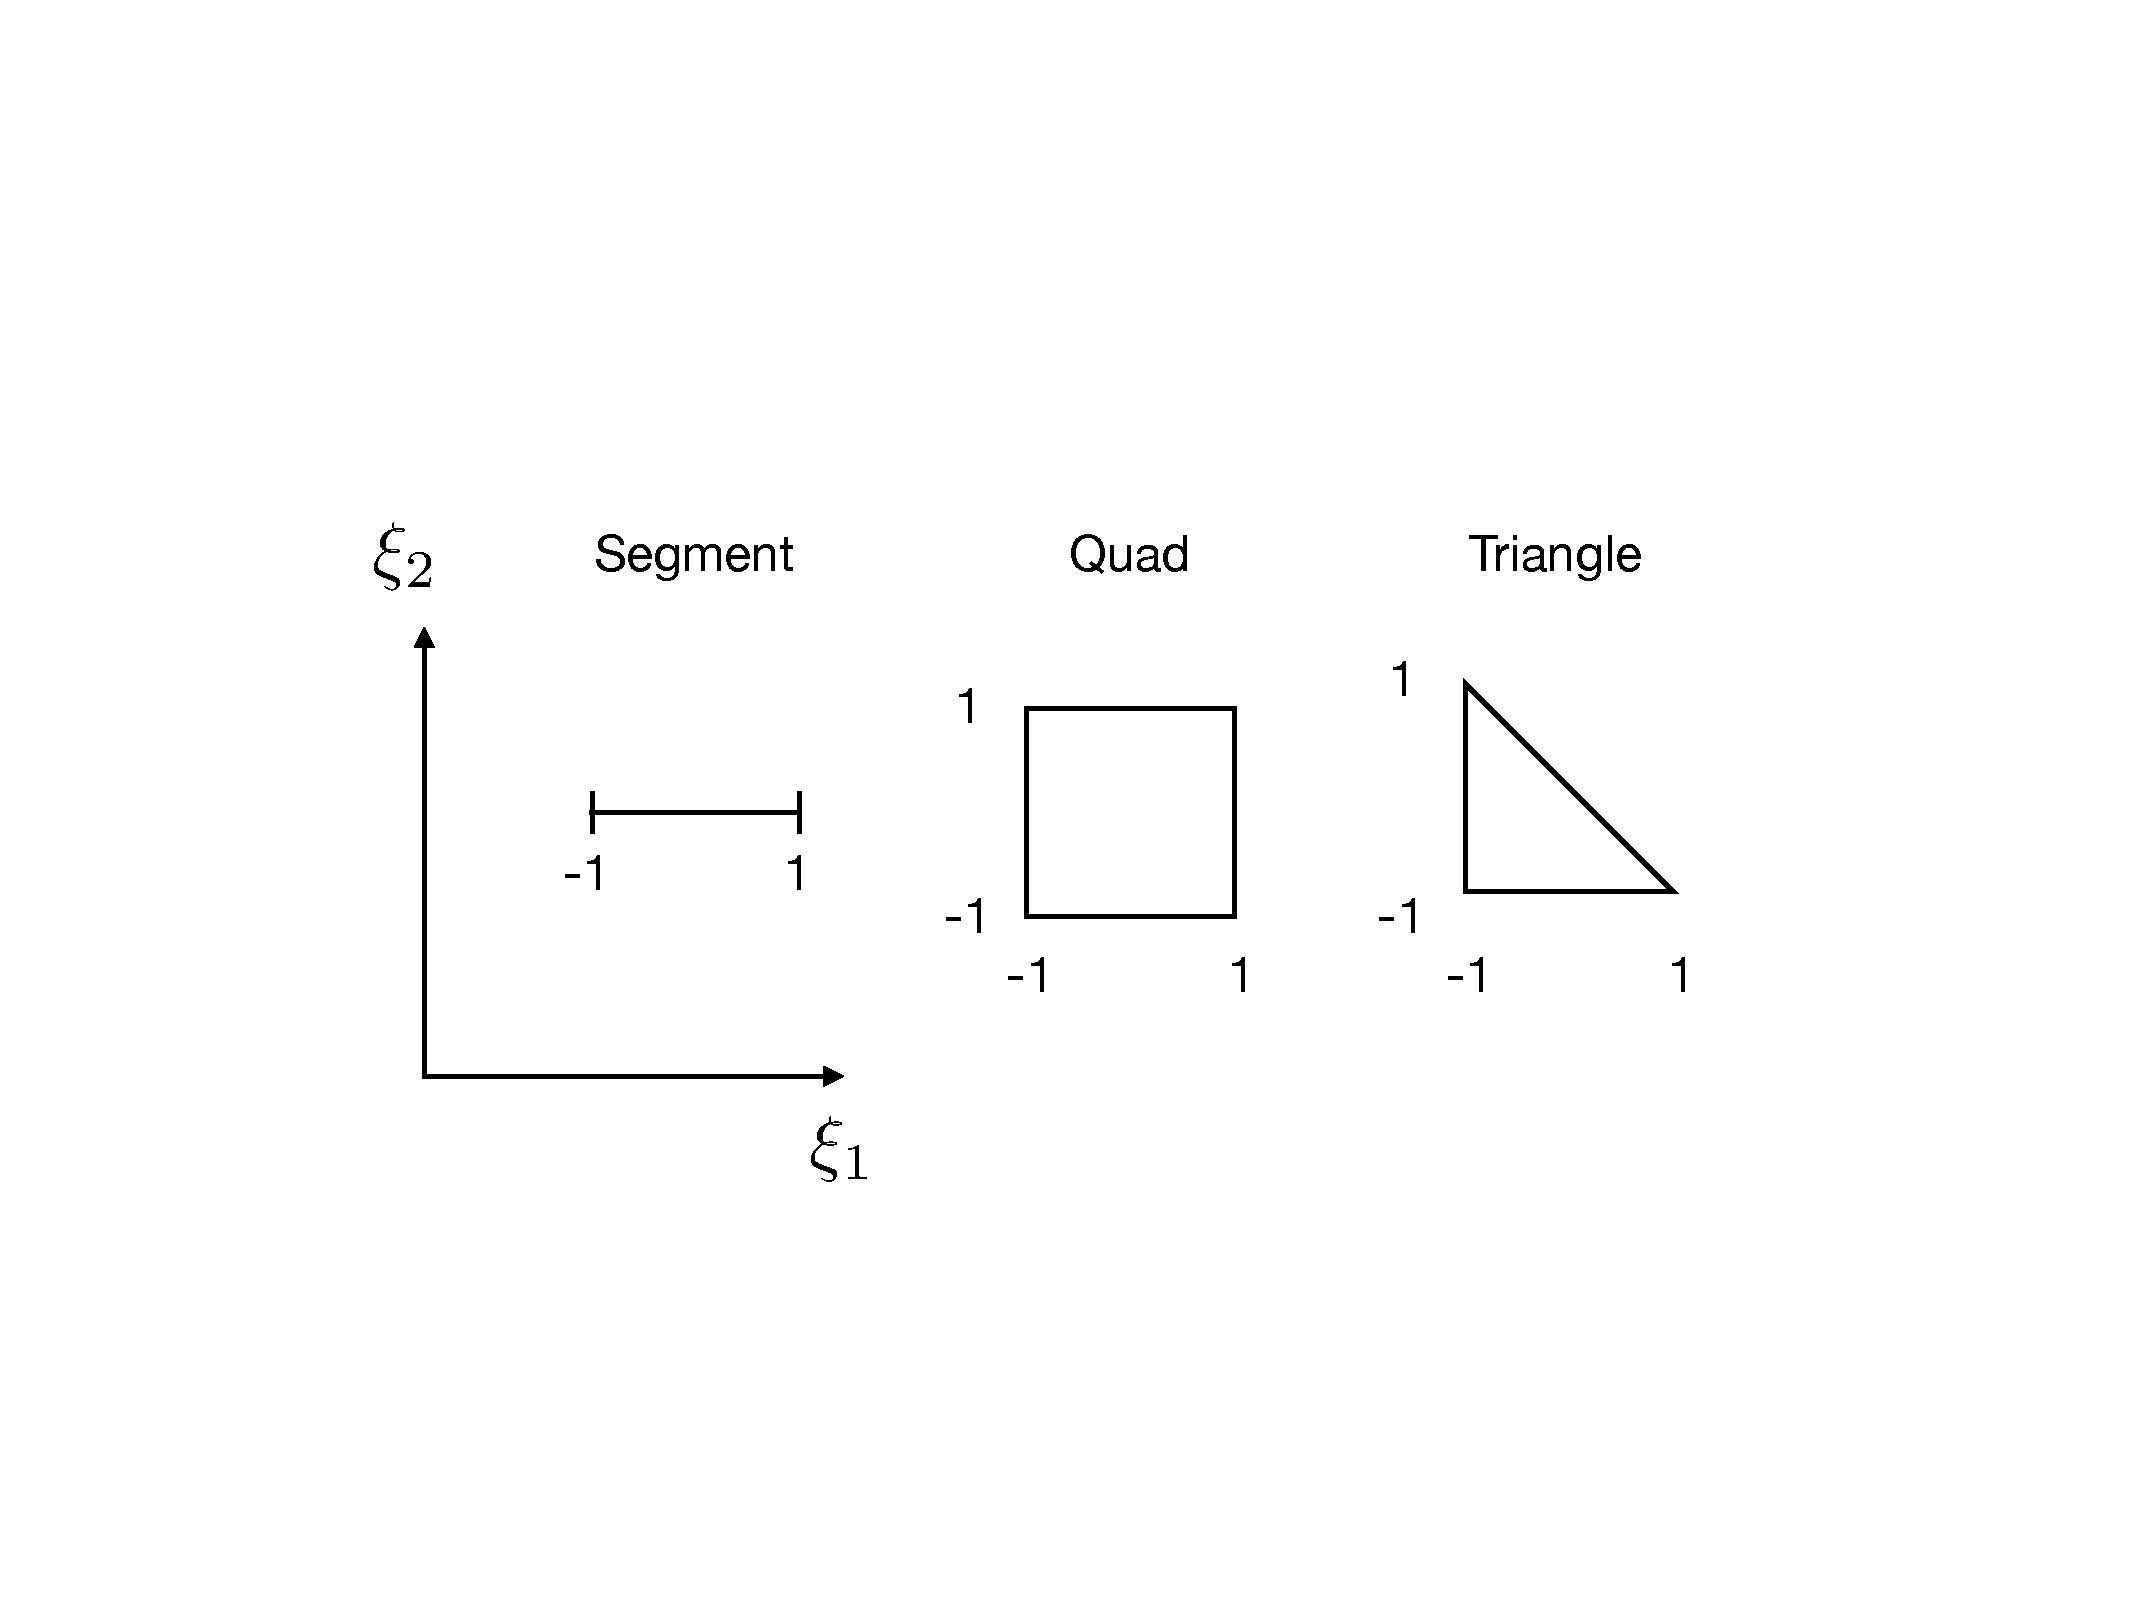
\includegraphics[width=4in]{img/refelement.pdf}
\caption{Example of the 1D and 2D reference space elements (segment, quad and triangle).}
\label{stdregions:refelement}
\end{figure}

The standard quad and standard hexahedra (shorthanded 'hex') are geometrically tensor-product constructions defined
on $[-1,1]^d$ for $d=2$ and $d=3$ respectively.  The standard triangle is constructed by taking $\xi_1 \in [-1,1]$ and taking $\xi_2 \le -\xi_1$.
The standard tetrahedra (shorthanded 'tet') is built upon the standard triangle and has all four faces being triangles, with the two
triangles along the coordinate directions looking like the standard triangle.  The standard prism consists of a standard 
triangle along the $\xi_1--\xi_2$ plane extruded into the third direction (yielding three quadrilateral faces).  The standard
pyramid consists of a standard quadrilateral at the base with four triangular faces reaching up to its top vertex  We show this
pictorially in Figure \ref{stdregions:3dshapes}.


\begin{figure}[htb]
\centering
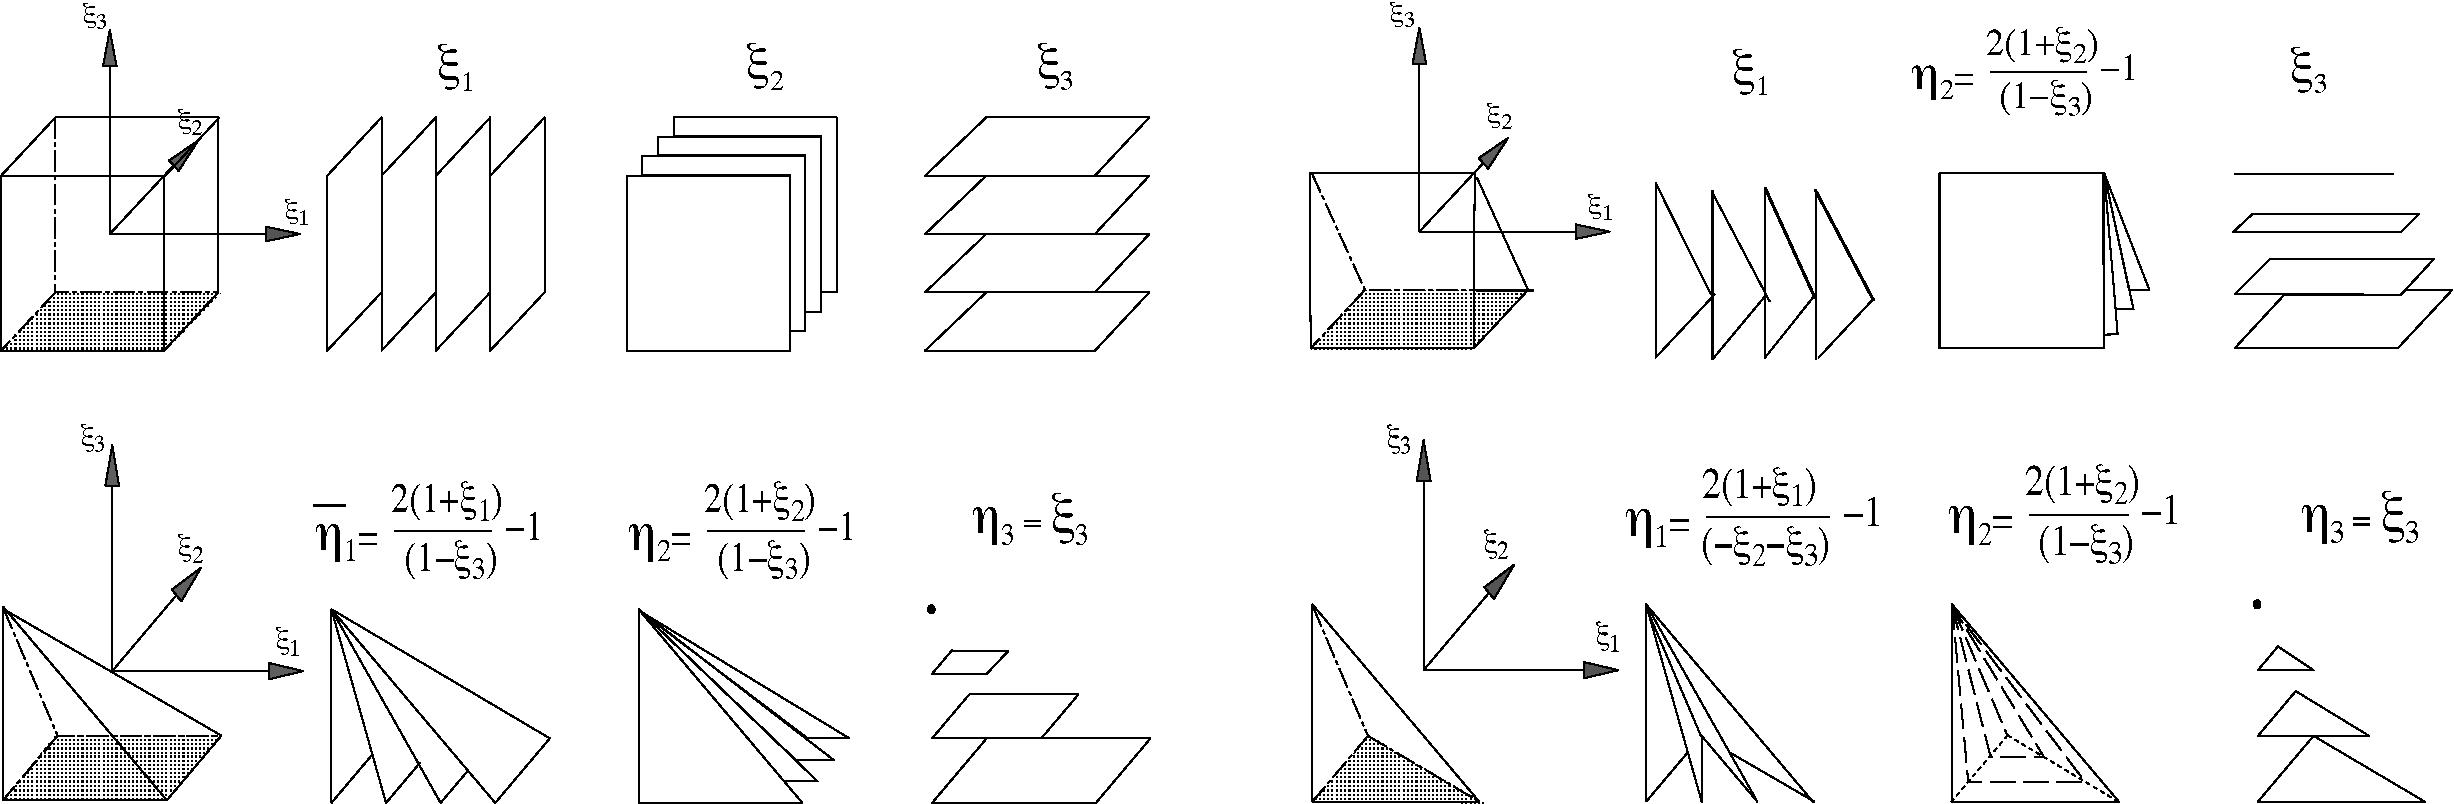
\includegraphics[width=4in]{img/LocalCoords.pdf}
\caption{Hexahedron to tetrahedron transformation showing how to go from an element on $[-1,1]^3$ (i.e. a standard hexahedron) to the three other element types which are subsets on $[-1,1]^3$.  Image taken from \cite{KaSh05}.}
\label{stdregions:3dshapes}
\end{figure}

Regardless of the particular element type, we use the fact one can build polynomial spaces over these geometric 
objects.  In the case of triangles and tetrahedra, these are polynomial spaces in the mathematical sense, i.e. $\mathcal{P}(k)$
spaces.  In the case of quadrilaterals and hexahedra, these are bi-- and tri-polynomial spaces, i.e. $\mathcal{Q}(k)$. 
In the case of prisms and pyramids, the spaces are more complicated and are a mixture in some sense of these spaces, but
they are indeed polynomial in form.  This allows us to define differentiation exactly and to approximate integrals
exactly up to machine precision.

In what is to follow, we describe (1) how you can build differentiation and integration operators over standard regions by mapping
them to a domain over which you can exploit index separability; and then (2) how you can build differentiation and integration operators
natively over various standard region shapes.  The former allows one to benefit from tensor-product operators, and is at present the 
primary focus of all {\nek} operators.  The latter as implemented for nodal element types is currently an {\em is-a} class definition 
extended from the (tensor-product-based) standard element definitions.



%%%%%%%%%%%%%%%%%%%%%%%%%%%%%%%%%%%%%%%%
\subsection{Reference Element Transformations That Facilitate Separability}

Differentiation and integration over the standard elements within {\nek}, in general, always try to map things back to tensor-product
(e.g. tensor-contraction indexing).  This allows one to transform operators that would normally have iterators that go from $i=0,\ldots,N^d$ 
where $d$ is the dimension of the shape to operators constructed with $d\cdot N$ operations (i.e., the product of one-dimensional operations).

As an example (to help the reader gain an intuitive understanding), consider the integration of a function $f(\vec{x})$ over a 
hexahedral element.  If we had a quadrature rule in 3D that needed $N^d$ points to integrate this function exactly, we would
express the operation as:

\begin{equation*}
\int_E f(\vec{x})\, d\vec{x} \approx \sum_{i=0}^{N^d} \omega_{i}\, f(\vec{z}_i)
\end{equation*}

\noindent where $E$ denotes our $d$-dimensional element and the set $Q = \{\vec{z}_i,\omega_i\}$ denotes the set of 
points and quadrature weights over the element $E$.  Now, suppose that both our function $f(\vec{x})$ and our $Q$ were
separable: that is, $f(\vec{x})$ can be written as $f_1(x_1)\cdot f_2(x_2)\cdot f_3(x_3)$ where $\vec{x} = (x_1,x_2,x_3)^T$
and $Q$ can we written in terms of 1D quadrature: $\vec{z}_i = z^{(1)}_{i_1}\cdot z^{(2)}_{i_2} \cdot z^{(3)}_{i_3}$ with
the index handled by an index map $\sigma$ defined by $i=\sigma(i_1,i_2,i_3)= i_1 + N\cdot i_2 + N^2 \cdot i_3$,
and similarly for the weights $\omega_i$.  We can then re-write the integral above as follows:

\begin{eqnarray*}
\int_E f(\vec{x})\, d\vec{x} &=& \int_E f(x_1)\cdot f(x_2) \cdot f(x_3)\,dx_1\,dx_2\,dx_3 \\
&\approx & \sum_{i=0}^{N^d} \omega_{i}\, f(\vec{z}_i) \\
&=& \sum_{i_1=0}^N \sum_{i_2=0}^N \sum_{i_3=0}^N \omega_{\sigma(i_1,i_2,i_3)}\, [f(z^{(1)}_{i_1})\cdot f(z^{(2)}_{i_2}) \cdot f(z^{(3)}_{i_3})] \\
&=& \left[ \sum_{i_1=0}^N \omega_{i_1}\,f(z^{(1)}_{i_1})\right]\cdot \left[ \sum_{i_2=0}^N \omega_{i_2}\,f(z^{(2)}_{i_2})\right] \cdot \left[ \sum_{i_3=0}^N \omega_{i_3}\,f(z^{(3)}_{i_3})\right]
\end{eqnarray*}

As you can see, when the functions are separable and the quadrature (or collocating points) can be written in separable form, we
can take $\mathcal{O}(N^d)$ operators and transform them into $\mathcal{O}(d\cdot N))$ operators.  The above discussion is
mainly focusing on the mathematical transformations needed to accomplish this; in subsequent sections, we will point out the 
memory layout and index ordering (i.e. now $\sigma$ is ordered and implemented) to gain maximum performance.

The discussion of tensor-product operations on quadrilaterals and hexahedra may seem quite natural as the element construction
is done with tensor-products of the segment; however, how do you create these types of operations on triangles (and anything
involving triangles such as tetrahedra, prisms and pyramids)?  The main mathematical building block we use that allows such
operators is a transformation due to Duffy \cite{Duffy82}, which was subsequently used by Dubiner \cite{Dubiner91} in the context
of finite elements  and was extended to general polyhedral types by Ainsworth \cite{AinsworthAD11,Ainsworth14}.

An image denoting the Duffy transformation is shown in Figure \ref{stdregions:duffy}.  On the left is an example of the
right-sided standard triangle with coordinate system $(\xi_1,\xi_2)$, and on the right is the separable tensor-product
domain with coordinates $(\eta_1,\eta_2)$.  We often refer to this transformation as ``collapsed coordinates" as it
appears as the ``collapsing" of a quadrilateral domain to a triangle.    Note that the edge along $\eta_1 = 1$ on
the quadrilateral collapses down to the single point $(\xi_1,\xi_2)=(1,1)$.  This, in general, does not cause issues
with our integration over volumes as this is a point of measure zero.  However, special case will need be taken when
doing edge integrals.  We will make it a point to highlight those places in which special care is needed.

\begin{figure}[htb]
\centering
\includegraphics[width=4in]{img/afg002.pdf}
\caption{Duffy mapping between a right-sided triangle and a square domain.}
\label{stdregions:duffy}
\end{figure}


With the 2D Duffy transformation in place, we can actually create all four 3D element types from the starting point
of a hexahedra (our base tensor-product shape).  One collapsing operation yields a prism.  The second collapsing
operation yields a pyramid.  Lastly, a final collapsing operation yields a tetrahedra.  A visual representation of these
operations are shown in Figure \ref{stdregions:3Dduffy}.

\begin{figure}[htb]
\centering
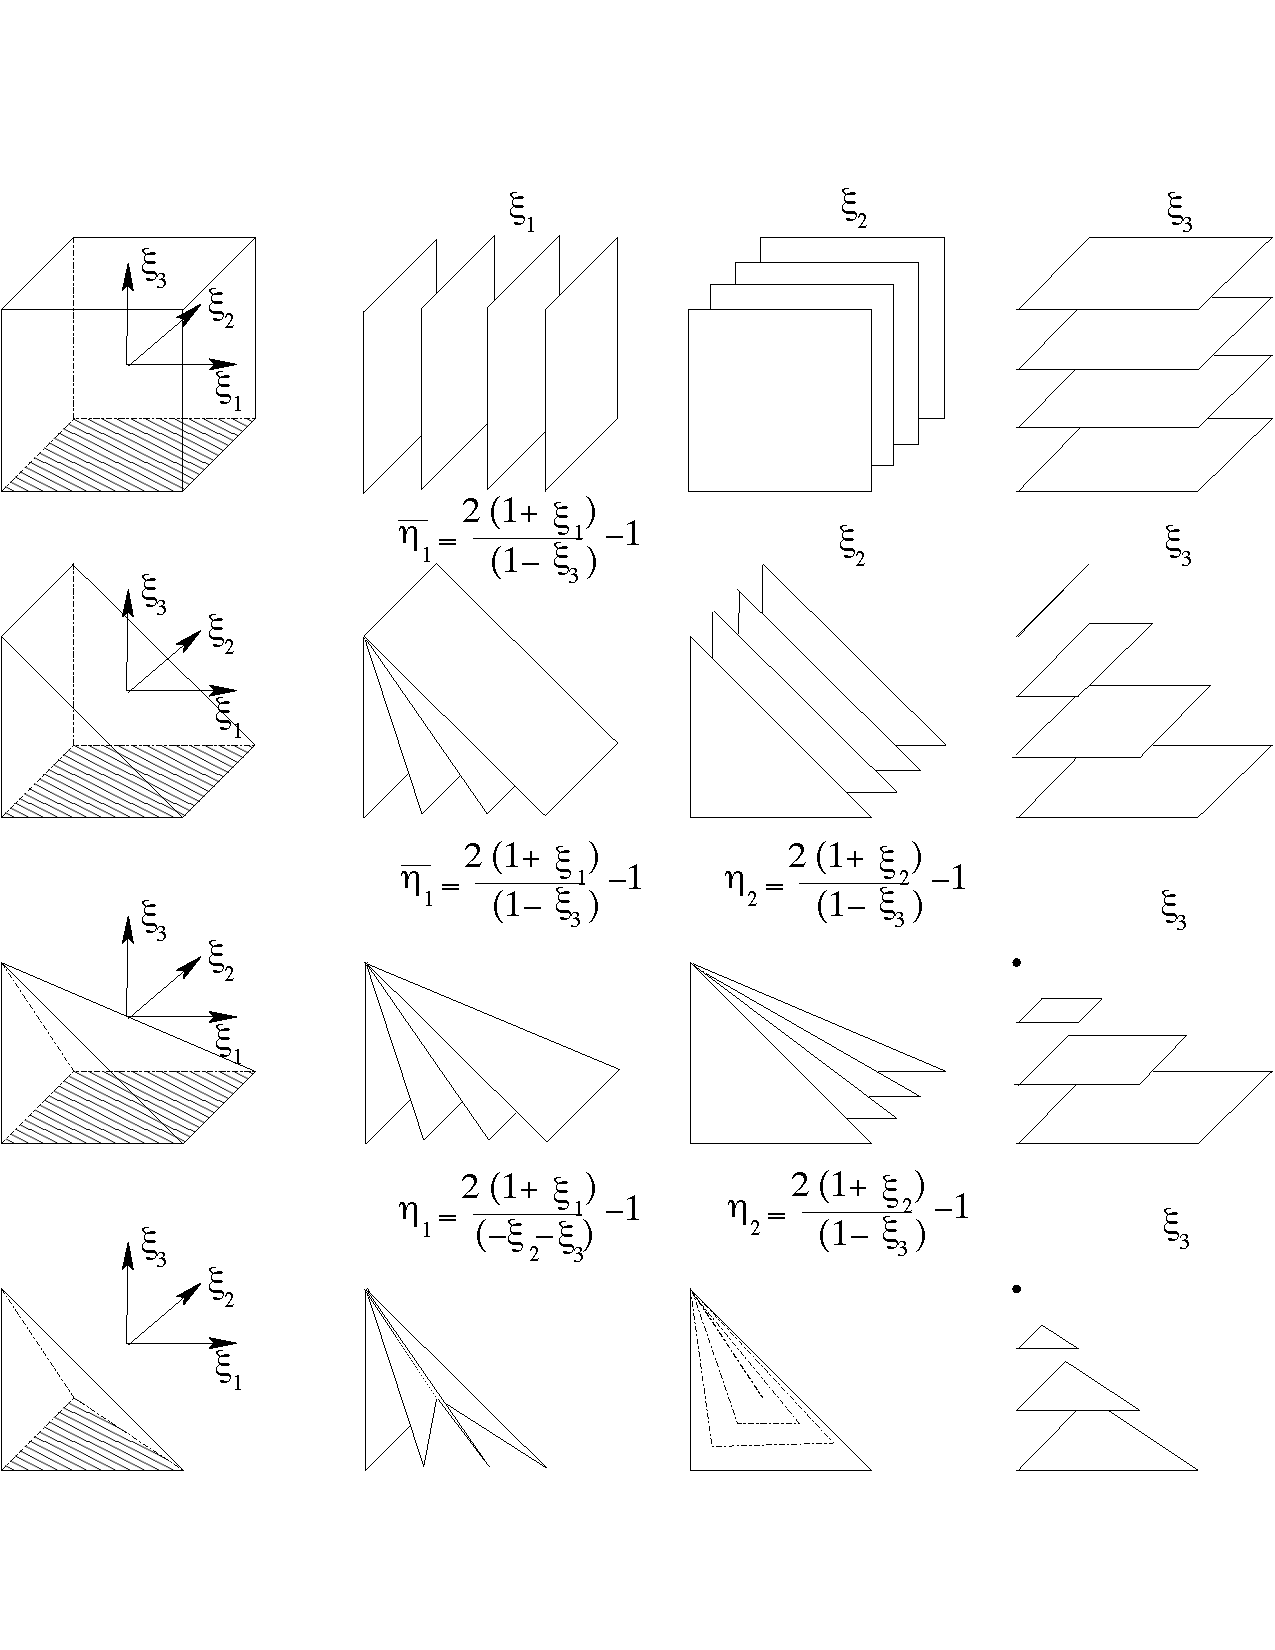
\includegraphics[width=4in]{img/3dcoords.pdf}
\caption{Duffy mapping application to generate all the 3D element types.  Image taken from \cite{KaSh05}.}
\label{stdregions:3Dduffy}
\end{figure}

This is meant merely to be a summary of tensor-product operations, enough to allow us to discuss the basic
data types and algorithms within {\nek}.  If more details are needed, we encourage the reader to consult
Karniadakis and Sherwin \cite{KaSh05} and the references therein.

%%%%%%%%%%%%%%%%%%%%%%%%%%%%%%%%%%%%%%%%
\subsection{Reference Elements On Primitive Geometric Types}

Although the primary backbone of {\nek} is tensor-product operations across all element types through the 
use of collapsed coordinates, we have implemented two commonly used non-tensorial basis set definitions.  
These are based upon Lagrange polynomial construction from a nodal (collocating) point set.  As derived
element types (in the $C++$ sense), we have implemented NodalStdTriangle (and Tet) based upon
the electrostatic points of Hesthaven \cite{Hesthaven98} and the Fekete points of 
Taylor and Wingate \cite{TaylorW99,TaylorWV00}.

Although these types of elements, at first glance, might seem to be ``sub-optimal" (in terms of operations), there
are various reasons why people might choice to use them.  For instance, the point set you use for defining 
the collocation points dictates the interpolative projection operator (and correspondingly the properties of that
operator) -- an important issue when evaluating boundary conditions, initial conditions and for some non-linear operator
evaluations.  Within the {\nek} team, we started an examination of this within the paper by 
Kirby and Sherwin \cite{KirbyS06}.  There has since been various papers in the literature (beyond the scope of this
developer's guide) that give the pros and cons of tensor-product (separable) and non-tensor-product element
types.  

